\newpage
\section{Successioni}
\begin{definition}[Successione]
Una successione\footnote{Nelle successioni si è soliti scrivere n al posto di x come simbolo per la variabile ess. $f(n)$} è una funzione $f: S\to \mathbb{R}$ dove S è una semiretta di $\mathbb{N}$, cioè $S = \{n \in \mathbb{R}\:|\: x\geq n_0\}$ per qualche $n_0$.
\end{definition}

\begin{example}
Consideriamo $f(n) = n^2$ con $S = \mathbb{N}$.
\end{example}
\begin{wrapfigure}[6]{l}{6cm}
    \vspace{-20pt}
    \centering
    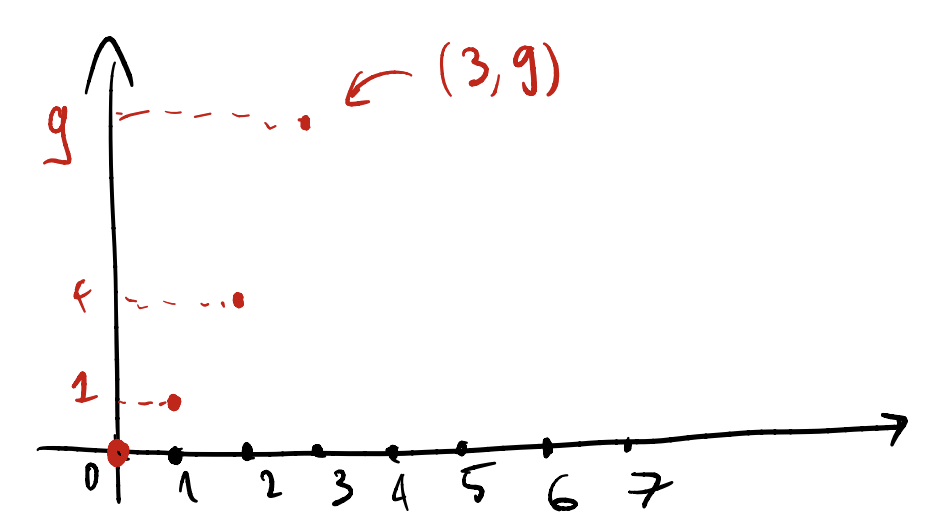
\includegraphics[width=5cm]{images/esempio-successione-1.png}
\end{wrapfigure}
Da questa funzione posso calcolare tutti i valori: $f(0) = 0^2 = 0$, $f(1) = 1^2 = 1$, $f(2) = 2^2 = 4$\\\\
E possibile disegnare un grafico di una successione che è composto da una serie di punti sparsi.\\

\begin{example}
$f(n) = \frac{1}{n}$, come S non posso prendere tutti i naturali perché con 0 non ha senso quindi $S = \{n \in \mathbb{N} \: |\: n \geq 1\}$.  $f(1) = \frac{1}{1}=1$, $f(2) = \frac{1}{2}$, $f(3) = \frac{1}{3}$.
\end{example}

\subsection{Notazione}
Nelle successioni invece di scrivere $f(n)$ di solito una successione si denota con $a_n$. Negli esempio di prima si sarebbe: $a_n = n^2$, $a_n = \frac{1}{n}$.\\
L'intera successione si denota con $\{a_n\}$ oppure $\{a_n\}_{n\in \mathbb{N}}$, $\{a_n\}_{n\in S}$.
\begin{example}
$a_n = \frac{1}{n-5}$. La formula ha senso per $n\neq 5$, quindi si può prendere $S = \{n \in \mathbb{N} \:|\: n\geq 6\}$ (avrei anche potuto prendere $n \geq 7$ o $n \geq 8$).
\end{example}

\begin{example}
$a_n = \sqrt{5 - n}$. La formula ha senso se $5-n \geq 0$ cioè $n \leq 5$. Nessuna semiretta va bene perché in una successione n diventa sicuramente più grande ad un certo punto quindi non definisce una successione.
\end{example}

\subsection{Limiti di Successioni}
Come per le funzioni bisogna guardare come si comporta la successioni all'avvicinarsi ad un limite. L'unico limite che ha senso è il limite per $n\to +\infty$, perché $+\infty$ è l'unico punto di accumulazione di tutto il dominio (perché $S \subseteq \mathbb{N}$).
\begin{definition}[Limite di successione]
Si ha che $\lim\limits_{n\to +\infty}a_n = l$ se $\forall \:\: U$ intorno di l si ha che $\exists \: \overline{n}\in \mathbb{N}$ tale che $a_n \in U \:\: \forall \: n\geq \overline{n}$.\\
Si dice che $a_n$ converge a $l$ se $\lim\limits_{n\to +\infty}a_n = l$ e $l\in \mathbb{R}$ e che diverge a $\pm \infty$ se $\lim\limits_{n\to +\infty}a_n = \pm \infty$.
\end{definition}

\begin{figure}[h!]
\centering
\begin{subfigure}{.45\textwidth}
    \vspace{-15pt}
    \centering
    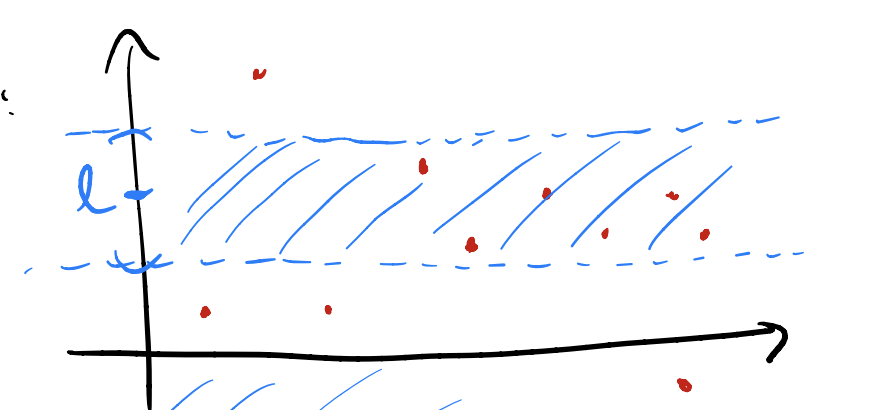
\includegraphics[width=5cm]{images/limite-successione-1.png}
    \caption{Graficamente se il limite è in $\mathbb{R}$ quindi $l \in \mathbb{R}$}
\end{subfigure}
\begin{subfigure}{.45\textwidth}
    \centering
    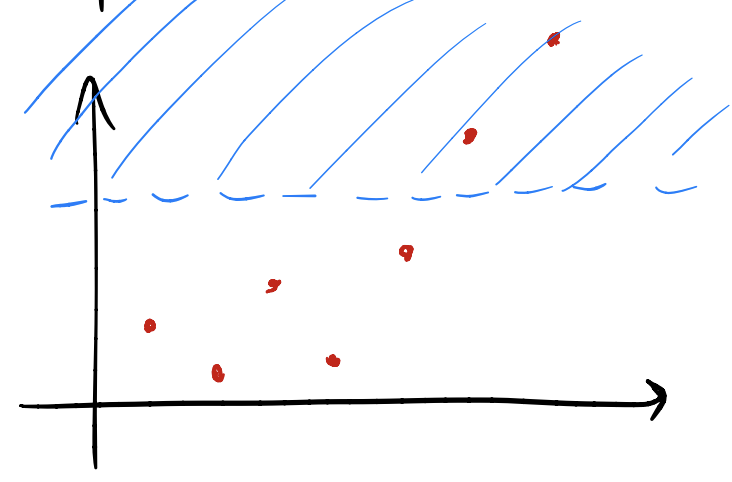
\includegraphics[width=4cm]{images/limite-successione-2.png}
    \caption{E con $l = +\infty$}
\end{subfigure}
\end{figure}

Esiste una \textbf{Terminologia} quando si parla di queste cose: se $P(n)$ è un predicato la cui verità dipende da $n\in \mathbb{N}$ (esempio: $P(n) =$ "n è pari") si dice che $P(n)$ è vero definitivamente se $\exists \: \overline{n}\in \mathbb{N}$ tale che $P(n)$ è vero $\forall n \geq \overline{n}$.\\
Quindi $\lim\limits_{n\to +\infty} a_n = l$ se $\forall \: U$ introno di l si ha che $a_n \in U$ definitivamente.

\subsection{Sottosuccessioni (estratte)}
\begin{definition}[Sottosuccessione]
Dato $a_n: S \to \mathbb{R}$ una successione, consideriamo $k_n: \mathbb{N} \to S$ strettamente crescente (cioè $k_n > k_m$ quando $n>m$), possiamo considerare la composizione $a_{k_n}$. Questa è una nuova successione detta sottosuccessione di $\{a_n\}$ (In pratica scegliamo solo un certo sottoinsieme di indici, in modo crescente).
\end{definition}

\begin{example}
Prendiamo la successione $a_n = \frac{1}{n}$.
\end{example}
\begin{wrapfigure}[4]{r}{6cm}
    \vspace{-40pt}
    \centering
    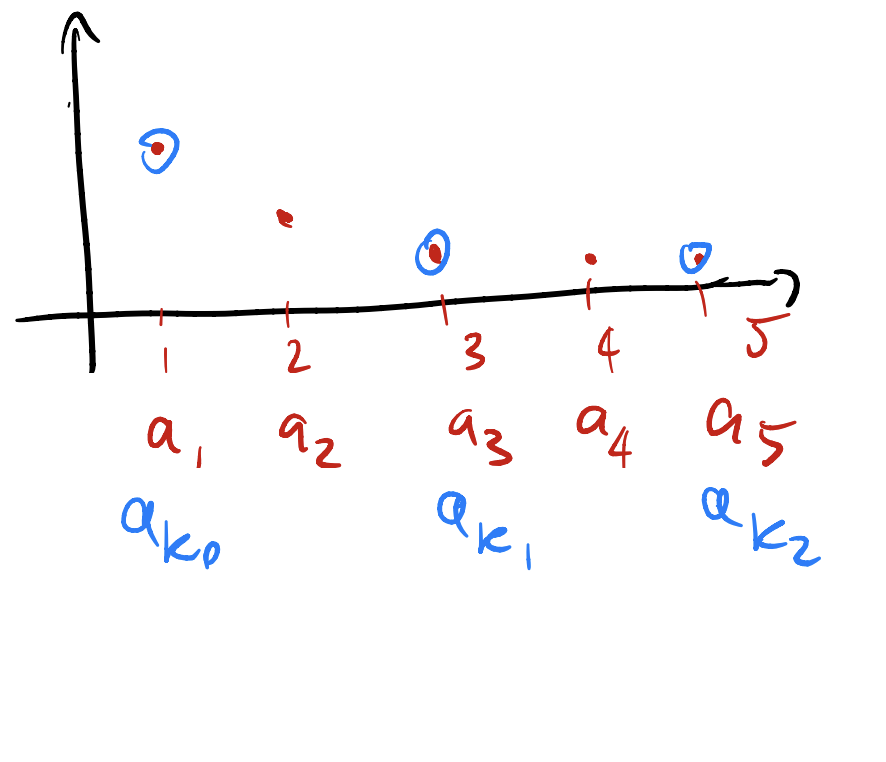
\includegraphics[width=5cm]{images/esempio-sottosuccessioni.png}
\end{wrapfigure}
Per avere una sottosuccessione prendo $k_n: \mathbb{N}\to S$,e prendo $n \mapsto 2n+1$. Abbiamo $a_{k_n} = \frac{1}{k_n} = \frac{1}{2n+1}$.\\
Quindi graficamente: \\
$a_{k_0} = \frac{1}{0+1} = 1$, $a_{k_1} = \frac{1}{2\cdot 1 +1} = \frac{1}{3} = a_3$, $a_{k_2} = \frac{1}{2 \cdot 2+1} = \frac{1}{5} = a_5$.\\\\
\begin{theorem}
Data una successione $\lim\limits_{n\to +\infty}a_n = l$ se e solo se vale $\lim\limits_{n\to +\infty}a_{k_n} = l$ per ogni sottosuccessione di $\{a_n\}$.
\end{theorem}
\hspace{-15pt} A volta si può usare per dimostrare che una successione non ha limite.
\begin{example}
$a_n= (-1)^h = \begin{cases}-1 & \text{se n è pari} \\ -1 & \text{se n è dispari} \end{cases}$ \\\\
Questo successione non ha limite e si dimostra con il teorema visto sopra. Infatti, consideriamo le sottosuccessioni $\{a_{2n}\}$ e $\{a_{2n+1}\}$ date da indici pari e dispari. \\
Abbiamo che $a_{2n} = (-1)^{2n} = (1)^n = 1$ che converge a 1 mentre, $a_{2n+1} = (-1)^{2n+1} = -1$ e quindi converge a -1. Visto che questi limiti esistono e sono diversi, segue dal teorema che $\{a_n\}$ non può avere limite.
\end{example}

\begin{observation}
Per i limiti di successioni valogono molti dei teoremi visti per le funzioni, ad esepio:
\begin{itemize}
    \item Formule per limiti di somme, prodotti, quozienti, esponenziali etc.
    \item Teorema di permanenza del segno.
    \item Teorema dei carabinieri.
    \item Teorema del confronto, ed altri...
\end{itemize}
\end{observation}

\begin{example}
Per esempio il teorema della permanenza del segno per le successioni dice: se abbiamo una successione che $\lim\limits_{n\to +\infty} a_n = l > 0$, allora $a_n > 0$ definitivamente.
\end{example}

\subsection{Monotonia}
\begin{definition}[Monotonia]
Una successione $\{a_n\}$ essa si dice:
\begin{itemize}
    \item \textbf{Debolmente crescente} se $n>m \Longrightarrow a_n \geq a_n$.
    \item \textbf{Strettamente crescente} se $n > m \Longrightarrow a > a_m$.
    \item \textbf{Debolmente decrescente} se $n > m \Longrightarrow a_n \leq a_m$.
    \item \textbf{Strettamente decrescente} se $n > m \Longrightarrow a_n < a_m$.
\end{itemize}
Successione è monotona quando vale una di queste 4 proprietà.
\end{definition}

\begin{observation}
$\{a_n\}$ è debolmente crescente se e solo se vale $a_{n+1} \geq a_n \forall \: n \in S$ (basta guardare termini successivi).\\
Infatti, se so che $a_{n+1} \geq a_n \forall \: n \in \mathbb{N}$, poi se $n > m$ allora $a_n \geq ... \geq a_{m+2} \geq a_{m+1} \geq a_{m}$.
\end{observation}

\begin{example}
Prendiamo $a_n=n^2$ e controlliamo che è strettamente crescente: vediamo che $a_{n+1} > a_n$. Infatti $a_{n+1} = (n+1)^2 = n^2 + 2n + 1$ e $a_n = n^2$ e quindi $n^2 + 2n + 1 > n^2 \Longleftrightarrow 2n+1 > 0$ che è vero $\forall \:n \in \mathbb{N}$.
\end{example}

\begin{theorem}
Se $\{a_n\}$ è monotona (cioè debolmente crescente o decrescente) allora ammette limite.
Se è debolmente crescente, il limite non può essere $-\infty$ e se Se è debolmente decrescente, il limite non può essere $+\infty$
\end{theorem}

\subsection{Limitatezza}
\begin{definition}[Limitatezza]
Una successione $\{a_n\}$ è \textbf{limitata superiormente} se $\exists\: M \in \mathbb{R}$ tale che $a_n \subseteq M \:\forall\: \in S$ e \textbf{limitata inferiormente} se $\exists \:m \in \mathbb{R}$ tale che $a_n \geq m \forall \: n \in S$ e \textbf{limitata} se è limitata sia inferiormente e superiormente. (immagine \ref{limitatezza-successioni})
\end{definition}

\begin{observation}
Una successione convergente (che ha limite finito) è limitata. Questo non è vero per funzioni di variabile reale.
\end{observation}

\begin{example}
$f(x) = \frac{1}{x}$, $f: (0,+\infty)\to \mathbb{R}$ abbiamo $\lim\limits_{x\to +\infty}f(x) = 0$ ma f non è limitata, perché $\lim\limits_{x\to 0^+}f(x) = +\infty$ però $a_n = \frac{1}{n}$ invece è limitata.
\end{example}

\begin{theorem}
Se $\lim\limits_{n\to +\infty}a_n = +\infty$, allora $\{a_n\}$ ha minimo (cioè $\exists \:n_{min} \in \mathbb{N}$ tale che $a_n \geq a_{n_{min}} \: \forall \:n \in S$). Se invece $\lim\limits_{n\to +\infty}a_n = -\infty$ allora $a_n$ ha massimo.  (immagine \ref{teorema-minimo})
\end{theorem}
\begin{figure}[h!]
\centering
\begin{subfigure}{.45\textwidth}
    \vspace{-25pt}
    \centering
    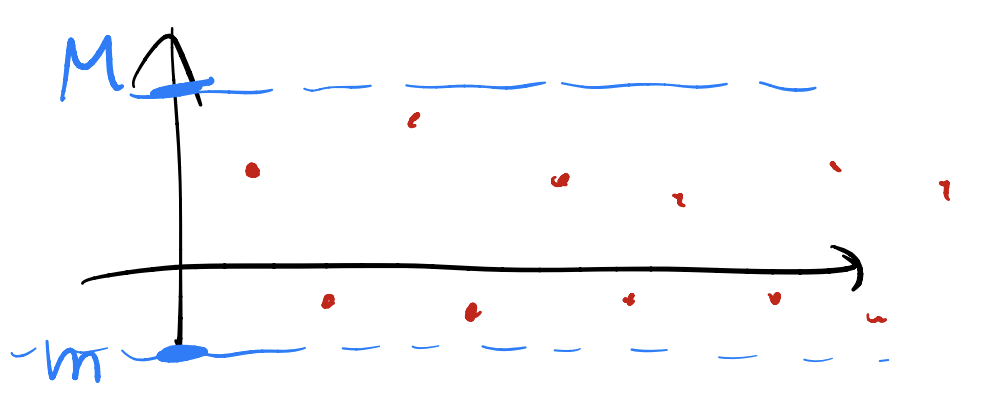
\includegraphics[width=5cm]{images/limitatezza-successioni.png}
    \caption{Graficamente definizione di limiti inf, sup}
    \label{limitatezza-successioni}
\end{subfigure}
\begin{subfigure}{.45\textwidth}
    \vspace{-15pt}
    \centering
    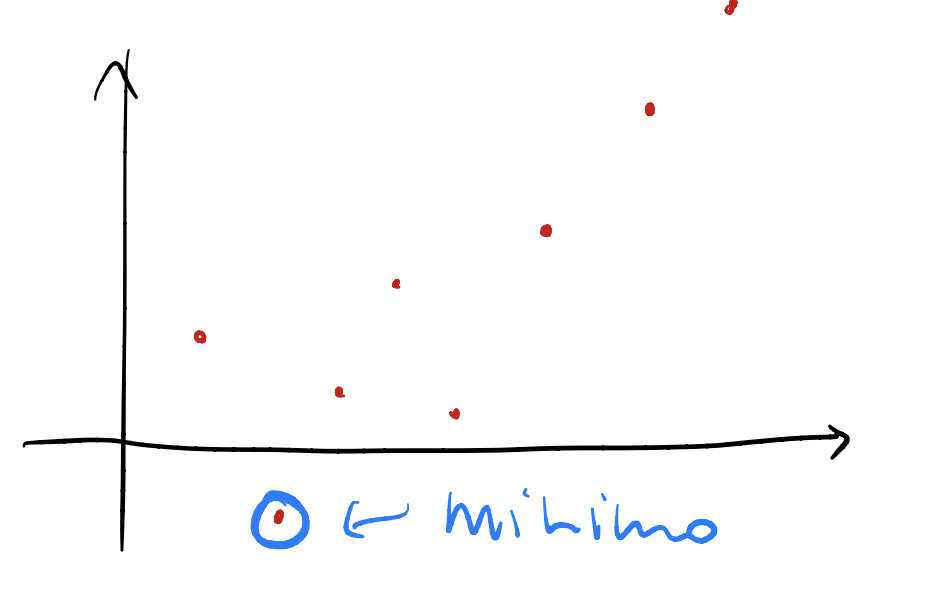
\includegraphics[width=4cm]{images/teorema-minimo.png}
    \caption{Graficamente teorema minimo massimo}
    \label{teorema-minimo}
\end{subfigure}
\caption{Raffigurazione di definizione limitatezza e teorema minimo massimo}
\end{figure}
\hspace{-15pt}Ci si può chiedere come domanda se una successione $\{a_n\}$ è limitata, necessariamente massimo e minimo? La risposte è no.
\begin{example}
Se prendiamo $a_n = \frac{1}{n}$ è limitata: $1 \geq \frac{1}{n} > 0$ ma non ha minimo. $max\{a_n\} = 1$ e $inf\{a_n\} = 0$ (uguale a $\lim\limits_{n\to +\infty} a_n$). Non ha minimo perché non esiste $n \in \mathbb{N}$ tale che $\frac{1}{n} = 0$
\end{example}
\hspace{-15pt}Inoltre è possibile chiedersi se $\{a_n\}$ è limitata, esiste almeno uno tra massimo minimo? E la risposta anche in questo caso è no.
\begin{example}
Prendiamo $a_n = (1-\frac{1}{n})(-1)^n = \begin{cases}1-\frac{1}{n} & \text{per n pari} \\ -(1 - \frac{1}{n}) & \text{per n dispari}\end{cases}$
\end{example}
\begin{figure}[h!]
\centering
\begin{subfigure}{.3\textwidth}
    \vspace{-25pt}
    \centering
    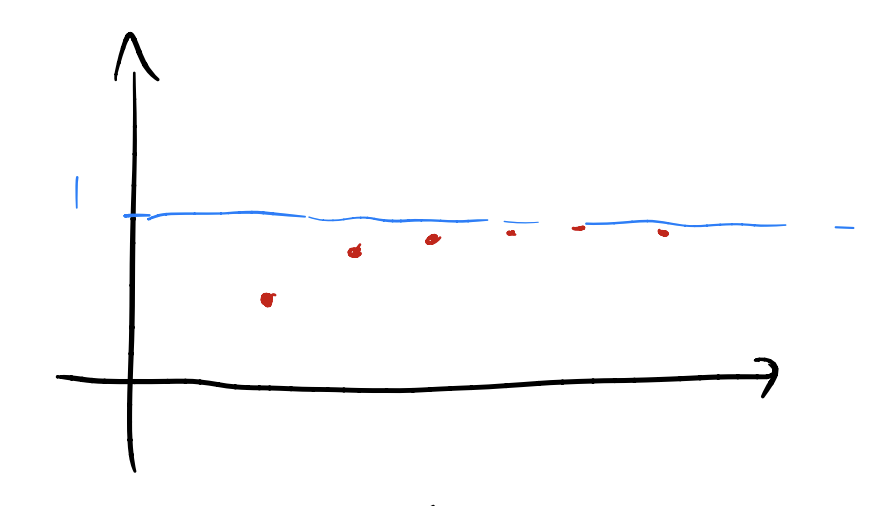
\includegraphics[width=4.5cm]{images/esempio-mas-min-succesioni-1.png}
    \caption{n pari}
\end{subfigure}
\begin{subfigure}{.3\textwidth}
    \centering
    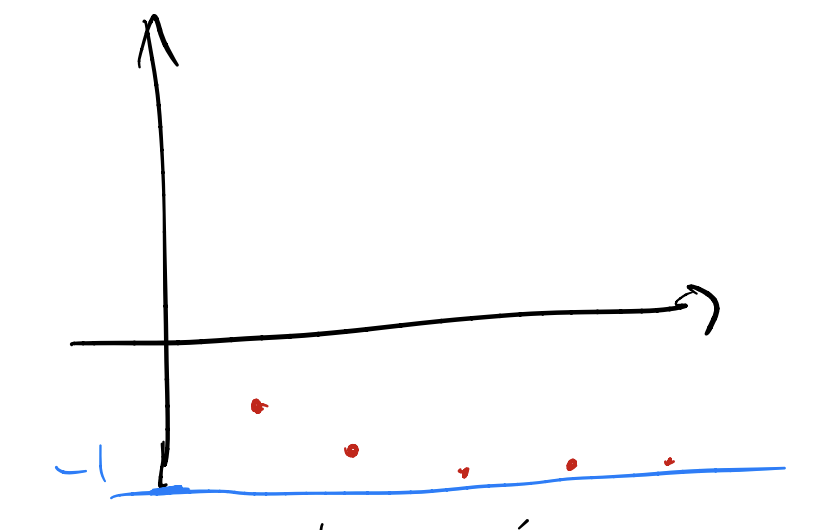
\includegraphics[width=4cm]{images/esempio-mas-min-succesioni-2.png}
    \caption{n dispari}
\end{subfigure}
\begin{subfigure}{.3\textwidth}
    \centering
    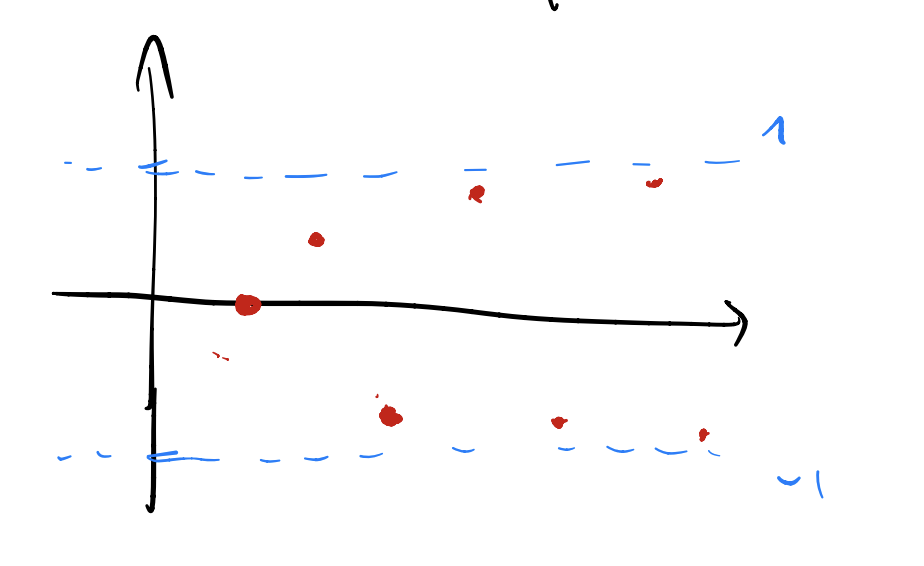
\includegraphics[width=4cm]{images/esempio-mas-min-succesioni-3.png}
    \caption{Complessivamente}
\end{subfigure}
\end{figure}
\hspace{-15pt}Complessivamente possiamo vedere la la successione oscilla avvicinandosi con $sun\{a_n\} = 1$ e $inf\{a_n\} = -1$, e non esistono massimo e minimo, anche se $a_n$ è limitata, visto che $-1 < a_n < 1$.

\newpage
\begin{example}
Prendiamo $a_n = \frac{(-1)^n}{n}$ e ci chiediamo se ha limite e sa ha massimo e o minimo.
\end{example}
\begin{wrapfigure}[4]{l}{6cm}
    \vspace{-15pt}
    \centering
    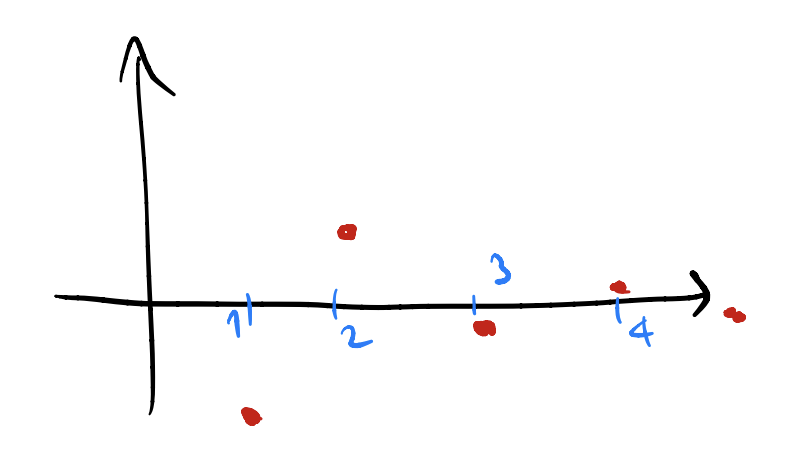
\includegraphics[width=5cm]{images/esempio-mas-min-successioni-4.png}
\end{wrapfigure}
Abbiamo che $\lim\limits_{n\to +\infty} = 0$. Infatti abbiamo che $-\frac{1}{n} \leq a_n \leq \frac{1}{n}$ e visto che $\lim\limits_{n\to +\infty}-\frac{1}{n}=\lim\limits_{n\to +\infty}\frac{1}{n} = 0$ per il teorema dei carabinieri abbiamo che $\lim\limits_{n\to +\infty}a_n = 0$. Quindi ha massimo e minimo il massimo è in $n=2$ ed il minimo in $n=1$.\\\\

\begin{theorem}
Se ho usa successione che converge $\lim\limits_{n\to +\infty}a_n = l$ finito allora:
\begin{itemize}
    \item $\exists \: \overline{n}\in \mathbb{N}$ tale che $a_{\overline{n}} \geq l \Longrightarrow \{a_n\}$ ha massimo.
    \item $\exists \: \overline{n}\in \mathbb{N}$ tale che $a_{\overline{n}} \leq l \longrightarrow \{a_n\}$ ha minimo.
\end{itemize}
\end{theorem}

\subsection{Legame tra limiti di funzione e successioni}
\begin{theorem}
Prendiamo una funzione definita in $A \subseteq \mathbb{R}$ sottoinsieme $f:A \to \mathbb{R}$, e $x_0 \in acc(A)$. Allora abbiamo che $\lim\limits_{x\to x_0}f(x) = l$ se e solo se $\lim\limits_{n\to +\infty}f(a_n) = l$ per ogni successione $\{a_n\}\subseteq A$ tale che $\lim\limits_{n\to +\infty}a_n = x_0$ e $a_n \neq x_0$ definitivamente.
\end{theorem}
\begin{wrapfigure}[2]{r}{6cm}
    \vspace{-35pt}
    \centering
    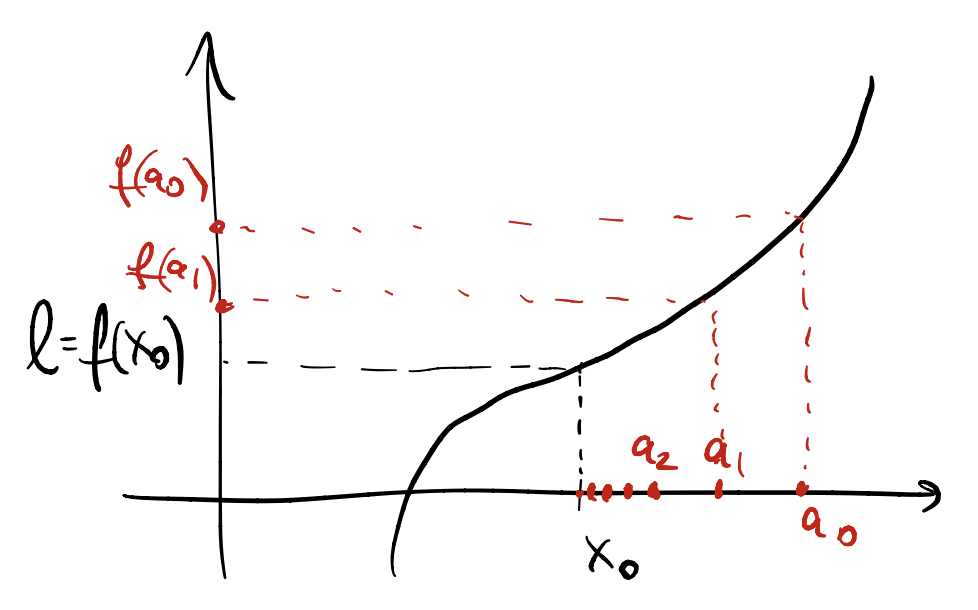
\includegraphics[width=4.7cm]{images/legame-lim-successioni-funzioni.png}
\end{wrapfigure}
Questo teorema a volte si può utilizzare per dimostrare che non esiste $\lim\limits_{x\to x_0}f(x)$.\\\\
\begin{example}
Dimostriamo che non esiste $\lim\limits_{x\to +\infty}\sin(x)$.\\
Esibiamo due successioni $a_n, b_n$ che tendono a $+\infty$,  tali che $\lim\limits_{n\to +\infty}\sin(a_n)$ e $\lim\limits_{n\to +\infty}\sin(b_n)$ esistono, ma sono diversi.\\
Prendo $a_n = n\pi$. Abbiamo $\lim\limits_{a\to +\infty}a_n = n\pi = +\infty$. Inoltre $\lim\limits_{n\to +\infty}\sin(a_n)= \lim\limits_{n\to +\infty}\sin(n\pi) = 0$ e $b_n = \frac{\pi}{2} + 2n\pi$. Di nuovo, $\lim\limits_{n\to +\infty}b_n = +\infty$ ma questa volta $\lim\limits_{n\to +\infty}\sin(b_n) = \sin(\frac{\pi}{2} + 2n\pi) = 1$.
\end{example}
\begin{wrapfigure}[4]{l}{6cm}
    \vspace{-15pt}
    \centering
    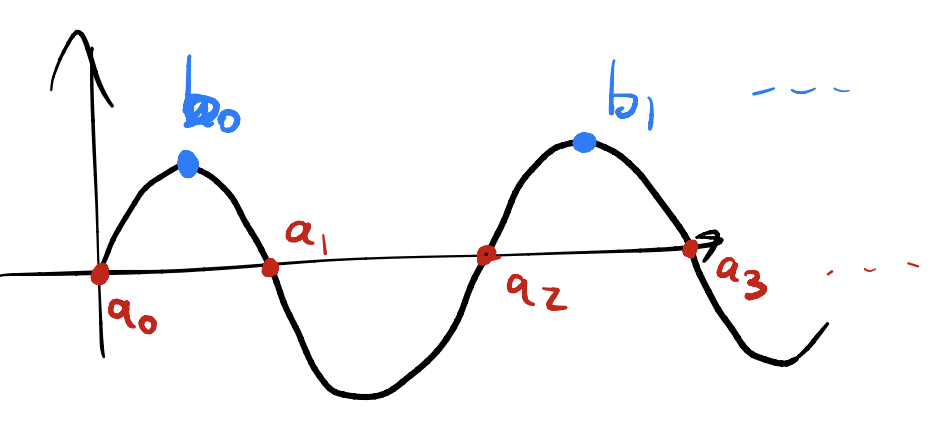
\includegraphics[width=5cm]{images/esempio-dim-con-legame-succ-fun.png}
\end{wrapfigure}

Per il teorema concludo che non esiste il $\lim\limits_{x \to +\infty}\sin(x)$
In particolare il teorema implica che se $\lim\limits_{x\to +\infty}f(x) = l$, allora $\lim\limits_{n\to +\infty}f(n) = l$. Attenzione che non è vero il viceversa.\\\\
\begin{example}
$f(x) = \sin(x\pi)$. Abbiamo $f(n) = \sin(n\pi) = 0$. Quindi $\lim\limits_{n\to +\infty}f(n) = 0$, ma non esiste $\lim\limits_{x\to +\infty}\sin(x\pi)$.
\end{example}

\subsection{Calcolo dei limiti di successioni}
\begin{theorem}
Se abbiamo due successioni $a_n \to l$ e $b_n \to l'$ allora $a_n + b_n \to l + l'$, $a_n \cdot b_n \to l \cdot l'$, $\frac{a_n}{b_n} \to \frac{l}{l'}$ (se $l' \neq 0$ e $b_n \neq 0$ definitivamente), $a_n^{n^n} \to l^{l'}$ (se $l>0$ e $a_n > 0$ definitivamente), se $a_n = c \forall\: n \in \mathbb{N}$ allora $\lim\limits_{n\to +\infty}a_n = c$.
\end{theorem}
\hspace{-15pt}Questo teorema vale solo se supponiamo che non vengono forme indeterminate che sono le stesse viste con le funzioni.
\begin{theorem}
Se $f: A \to \mathbb{R}$ e $x_0 \in acc(A)$ e $\lim\limits_{x\to x_0}f(x) = l$ e $a_n: S \to A$ tale che $a_n \to x_0$ e $a_n \neq x_0$ definitivamente allora $\lim\limits_{n\to +\infty}f(a_n) = l$. In particolare se $\lim\limits_{x\to +\infty}f(x) = l$, allora $\lim\limits_{n\to +\infty}f(n) = l$.
\end{theorem}

\begin{example}
Alcuni esempi di calcolo dei limiti con successioni:
\begin{itemize}
    \item $\lim\limits_{n\to +\infty}(n^2 + 2n)$. Partendo da $\lim\limits_{n\to +\infty}n = +\infty$ troviamo $(\lim\limits_{n\to +\infty}n^2) + \lim\limits_{n\to +\infty}(2n) = (\lim\limits_{n\to +\infty}n)(\lim\limits_{n\to +\infty}n) + 2 \lim\limits_{n\to +\infty}n = (+\infty) \cdot (+\infty) + 2(+\infty) = +\infty$.
    \item $\lim\limits_{n\to +\infty}(n^2 - 2n) = +\infty - \infty$ possiamo fare $n^2 - 2n = n(n-2) \to +\infty \cdot (+\infty) = +\infty$. Si poteva anche dire $f(x) = x^2 - 2x$ visto che $\lim\limits_{x\to +\infty} (x^2 - 2x)=+\infty$ allora $\lim\limits_{n\to +\infty}f(n) = +\infty$.
    \item $\lim\limits_{n\to +\infty}\frac{n^2 - 2n}{n} = +\frac{+\infty}{+\infty}$ possiamo però fare $\frac{n^2 - 2n}{n} = n-2 \to +\infty$.
    \item $\lim\limits_{n\to +\infty}e^n$, consideriamo $f(x) = e^x$, so che $\lim\limits_{x\to +\infty}e^x = +\infty$ quindi $\lim\limits_{n\to +\infty}f(n) = +\infty$.
    \item $\lim\limits_{n\to +\infty}n\cdot \sin\frac{1}{n} = +\infty \cdot 0$, pongo $f(x) = x \cdot \sin\frac{1}{x}$ e calcoliamo $\lim\limits_{x\to +\infty}x\cdot \sin\frac{1}{x} = \frac{\sin\frac{1}{x}}{\frac{1}{x}}$ e $\frac{1}{x} \to 0$ quando $x\to +\infty$, poniamo $t = \frac{1}{x}$ e viene $\lim\limits_{x\to +\infty}\frac{\sin{t}}{t} = 1$.\\\\
    Altro modo utilizzando taylor: poniamo $\sin{t} = t + o(t)$ per $t\to 0$ sostituisco $t=\frac{1}{n}$ (infatti $\frac{1}{n}\to 0$ quando $n\to +\infty$), po $\sin{\frac{1}{n}} = \frac{1}{n} + o(\frac{1}{n})$ quindi $n\cdot \sin{\frac{1}{n}} = n \cdot (\frac{1}{n} + o(\frac{1}{n})) = 1 + o(1) \to 1$ per $x\to +\infty$.
\end{itemize}
\end{example}

\begin{observation}
$f(n)$ può avere limite anche se $f(x)$ non c'è l'ha infatti per esempio:
$f(x) = \sin{\pi x}$ non ha limite per $x\to +\infty$ ma $f(n) = \sin{\pi n}$ ha limite. \\
Quindi il metodo di utilizzare la funzione può non sempre funzionare.
\end{observation}

\begin{example}
Ci chiediamo se esiste $\lim\limits_{n\to +\infty}\sin(n)$. Vediamo che il limite non esiste:\\
Chiediamo quando $\sin(x) \geq \frac{1}{2}$ in $[0,\pi]$ succede esattamente per $x \in [\frac{\pi}{6},\frac{5}{6}\pi]$. L'intervallo ha lunghezza $\frac{5}{6}\pi - \frac{1}{6}\pi = \frac{4}{6}\pi = \frac{2}{8}\pi > 2$. Quindi l'intervallo contiene almeno due numeri interi (in $\mathbb{N}$) e lo stesso vale per tutti gli traslati di multipli di $2\pi$.\\
Questo ci permette di costruire una successione crescete $h_n$ di numeri naturali tale che $\sin(h_n) \geq \frac{1}{2} \: \forall \: n \in \mathbb{N}$.
Questo mi dice che se esiste $\lim\limits_{n\to +\infty}\sin(n) = l$, allora sicuramente $l \geq \frac{1}{2}$ (conseguenza della permanenza del segno). \\
Posso fare lo stesso discorso partendo da $\sin(x) \leq -\frac{1}{2}$, e trovo che $l \leq -\frac{1}{2}$. Questo è assurdo, e mi dimostra che non esiste $\lim\limits_{n\to +\infty}\sin(n)$.
\end{example}

\begin{example}
$\lim\limits_{n\to +\infty}n^2 \cdot \sin{n}$, ci chiediamo se esiste il limite.\\
Considerando la successione dell'esempio precedente $h_n$, troviamo una sottosuccessione $h_n^2 \cdot \sin(h_n)$, $\sin(h_n) \geq \frac{1}{2}$ quindi $h_n^2 \cdot \sin(h_n) \geq \frac{1}{2}\cdot h_n^2 \to +\infty$. Se $k_n$ è una successione di naturali tale che $\sin(k_n) \leq -\frac{1}{2} \forall \: n$, abbiamo una sottosuccessione $k_n^2 \cdot \sin(k_n) \leq -\frac{1}{2}kn^2 \to +\infty$. Quindi ho due sottosuccessioni di $n^2\sin{n}$ che hanno limiti diversi. Segue che non esiste $\lim\limits_{n\to +\infty}n^2 \cdot \sin{n}$.
\end{example}

\begin{theorem}
Sia $\{a_n\}_{n \in \mathbb{N}}$ (nota \footnote{In questa scrittura ci sono tutti i numeri naturali}) una successione,e $\{a_{h_n}\}$ e $\{a_{k_n}\}$ due sottosuccessioni tale che $\{h_n \: | \: n \in \mathbb{N}\} \cup \{k_n \: | \: n \in \mathbb{N}\} = \mathbb{N}$. (si dice che le due sottosuccessioni "saturano tutti gli indici").\\
Se $\exists \: \lim\limits_{n\to +\infty}\_{h_n}$ e $\exists \lim\limits_{n\to +\infty}a_{k_n}$ e sono uguali, allora esiste anche $\lim\limits_{n\to +\infty}a_n$ ed è uguale agli altri due.
\end{theorem}
\hspace{-15pt}Un caso tipico in cui si utilizza questo teorema è quando si prendono gli indici pari e dispari.
\begin{example}
$\Large{\lim\limits_{n\to +\infty}\frac{(\log{n+1})^{(-1)^h}}{n^3}}$. Guardiamo gli indici pari $k_n = 2n$ con il quale ho $\frac{(\log(2n+1))^1}{(2n)=3} \to 0$, e poi guardiamo gli indici dispari $h_n = 2n+1$ dove viene $\frac{(\log(2n+1))^{-1}}{(2n+1)^3} = \frac{1}{(2n+1)^3\log(2n+1)} = \frac{1}{+\infty} = 0$ quindi le sottosuccessioni saturano tutti gli indici.\\
Usando il teorema concludiamo che $\Large{\lim\limits_{n\to +\infty}\frac{(\log{n+1})^{(-1)^h}}{n^3}} = 0$.
\end{example}

\subsubsection{Criterio del rapporto}
\begin{theorem}[Criterio del rapporto]
Sia $\{a_n\}$ una successione.  Se $a_n > 0$ definitivamente, e se esiste $\lim\limits_{n\to +\infty}\frac{a_{n+1}}{a_n} = l$ allora:
\begin{enumerate}
    \item Se $0 \leq l \leq 1$, allora $\lim\limits_{n\to +\infty} a_n = 0$.
    \item Se $l > 1$, allora $\lim\limits_{n\to +\infty}a_n = +\infty$.
\end{enumerate}
\end{theorem}

\begin{observation}
Se $l = 1$, non si può dire niente sul comportamento di $a_n$.
\end{observation}

\begin{example}
Esempi del criterio del rapporto con $l=1$:
\begin{itemize}
    \item Prendo $a_n = 1 \forall \: n \in \mathbb{N}$. Allora $\frac{a_{n+1}}{a_n} = \frac{1}{1} = 1 \to 1$ quindi $l=1$ e $a_n$ converge a 1.
    \item Con $a_n = n$. Allora $\frac{a_{n+1}}{a_n} = \frac{n+1}{n} \to 1$ quindi $l=1$ e $a_n \to +\infty$.
    \item Con $a_n = \frac{1}{n}$, di nuovo $\frac{a_{n+1}}{a_n} = \frac{n}{n+1} \to 1$ sempre $l=1$ e $a_n \to 0$.
\end{itemize}
\end{example}

\begin{example}
Esempi di applicazioni del criterio del rapporto:
\begin{itemize}
    \item $a_n = (\frac{1}{2})^n$. Usando il criterio $\frac{a_{n+1}}{a_n} = \frac{(\frac{1}{2})^{n+1}}{(\frac{1}{2})^n} = \frac{2^n}{2^{n+1}} = \frac{1}{2} = l$ e ho $0 \leq l \leq 1$. Quindi $a_n \to 0$.
    \item $a_n = 2^n$ (si può usare $f(x) = 2^x$ e il fatto che $\lim\limits_{x\to +\infty}2^x = +\infty$). Usiamo il criterio del rapporto quindi $\frac{a_n+1}{a_n} = \frac{2^{n+1}}{2^n} = 2 = l$ e con $l>2$ concludo che $a_n \to +\infty$.
    \item $a_n = n!$. Criterio del rapporto che $\frac{a_{n+1}}{a_n} = \frac{(n+1)!}{n!} = \frac{(n+1)n!}{n!} = n+1 \to +\infty = l$ quindi $l>1$ e quindi $a_n \to +\infty$. In questo caso si poteva anche osservare che $n! > n$ e $n \to +\infty$ quindi per confronto segue che $n! \to +\infty$.
\end{itemize}
\end{example}

\hspace{-15pt}Confronto di $n!$ con $n^k$, $b^n$, $n^n$:
\begin{itemize}
    \item \textbf{Potenza} ($n^k$) con ($k\geq 1$). Vogliamo guardare che $\lim\limits_{n\to +\infty}\frac{n!}{n^k} = \frac{+\infty}{+\infty}$ forma indeterminata.\\
    Usiamo quindi il criterio del rapporto per $a_n = \frac{n!}{n^k}$. Ho $\frac{a_{n+1}}{a_n} = \frac{(n+1)!}{(n+1)^k} \cdot \frac{n^k}{n!} = \frac{(n+1)!}{n!} \cdot \frac{n^k}{(n+1)^k} = (n+1) \cdot (\frac{n}{n+1})^k \to +\infty \cdot (1)^k = +\infty = l$ quindi $l > 1$.\\
    Segue che $\frac{n!}{n^k} \to +\infty$, quindi $n!$ "tende a $+\infty$ più velocemente di $n^k$".
    \item \textbf{Esponenziale} ($b^n$) con $b > 1$. $\lim\limits_{n\to +\infty} \frac{n!}{b^n} = \frac{+\infty}{+\infty}$ forma indeterminata. Guardiamo quindi il rapporto, per $a_n = \frac{n!}{b^n}$. Quindi abbiamo $\frac{a_{n+1}}{a_n} = \frac{(n+1)!}{b^{n+1}} \cdot \frac{b^n}{n!} = \frac{(n+1)!}{n!} \cdot \frac{b^n}{b^{n+1}} = (n+1)\cdot \frac{1}{b} \to +\infty = l > 1$. Segue che $\frac{n!}{b^n} \to +\infty$, quindi $n!$ tende a $+\infty$ più velocemente di $b^n$.
    \item \textbf{Esponenziale potentissimo} ($n^n$). Notare che $n^n \to +\infty$ ad esempio perché $n^n \geq n$ e $n\to +\infty$. Facciamo $\lim\limits_{n\to +\infty}\frac{n^n}{n!} = \frac{+\infty}{+\infty}$ forma indeterminata. Usiamo il criterio del rapporto per $a_n = \frac{n^n}{n!}$. $\frac{a_{n+1}}{a_n} = \frac{(n+1)^{n+1}}{(n+1)!}\cdot \frac{n!}{n^n} = \frac{n!}{(n+1)!} \cdot \frac{(n+1)^{n+1}}{n^n} = \frac{1}{n+1} \cdot \frac{(n+1)^{n+1}}{n^n} = (\frac{n+1}{n})^n = (1 + \frac{1}{n})^n$ che è un limite notevole che $\to e > 1$. (per vederlo ad esempio si può scrivere $(1 + \frac{1}{n})^n = e^{\log(1+\frac{1}{n})^n} = e^{n\cdot \log(1+\frac{1}{n})} = e^{n\cdot(\frac{1}{n} + o(\frac{1}{n}))} = e^{1 + o(1)} \to e^1 = e$). Quindi segue che $\frac{n^n}{n!} \to +\infty$ quindi $n^n$ tende a $+\infty$ più velocemente di $n!$.
\end{itemize}


\subsubsection{Criterio della radice}
\begin{theorem}
Se $a_n > 0$ definitivamente, e $\exists \lim\limits_{n\to +\infty}\sqrt[n]{a_n} = l$, allora:
\begin{enumerate}
    \item Se $0 \leq l < 1$, allora $\lim\limits_{n\to +\infty} a_n = 0$.
    \item Se $l > 1$, allora $\lim\limits_{n\to +\infty}a_n = +\infty$.
\end{enumerate}
\end{theorem}

\begin{observation}
Se $l=1$ non si può dire niente riguardo al comportamento di $a_n$ come sul criterio del rapporto.
\end{observation}

\begin{demostration}
Dimostrazione dei due casi del criterio della radice.
\begin{enumerate}
    \item Suppongo che $0 \leq l \leq 1$ e fisso un $m\in \mathbb{R}$ tale che $l < m < 1$. Visto che $\sqrt[n]{a_n}\to l$ definitivamente avrò $\sqrt[n]{a_n} < m$, quindi $a_n < m^n$. Ora visto che $m < 1$ abbiamo visto che $m^n \to 0$, quindi visto che $0 < a_n < m^n$ per il teorema dei carabinieri segue che $a_n \to 0$.
    \item Questo punto si fa analogo, se invece $l > 1$ scelto $m \in \mathbb{R}$ tale che $1 < m < l$. Visto che $\sqrt[n]{a_n} \to l$ avrò $\sqrt[n]{a_n} > m$ definitivamente segue che definitivamente ho $a_n > m^n$ e visto che $n > 1$ ho $m^n \to +\infty$. Per confronto segue che $a_n \to +\infty$. $\blacksquare$
\end{enumerate}
\end{demostration}

\subsubsection{Relazione fra criteri del rapporto e della radice}
\begin{theorem}[Relazione fra rapporto e radice]
Se $a_n > 0$ definitivamente e se $\exists \lim\limits_{n\to +\infty}\frac{a_{n+1}}{a_n} = l$, allora $\exists \lim\limits_{n\to +\infty}\sqrt[n]{a_n}$ ed è uguale a l.
\end{theorem}

\begin{observation}
Questo teorema è vero anche con $l=1$.
\end{observation}

\begin{observation}
Potrebbe esiste $\lim\limits_{n\to +\infty}\sqrt[n]{a_n}$ e non esistere il $\lim\limits_{n\to +\infty} \frac{a_{n+1}}{a_n}$ (quindi questo teorema vale solo per un verso e non il viceversa).
\end{observation}

\begin{example}
Alcuni esempi utilizzando quest'ultimo teorema.
\begin{itemize}
    \item Fissiamo un $a > 0$. Proviamo a calcolare $\lim\limits_{n\to +\infty} \sqrt[n]{a}$. (Si può fare in diversi modi come $\sqrt[n]{a} = a^{\frac{1}{n}} \to a^0 = 1$).
    Usiamo l'ultimo teorema $a_n = a$ successione costante. Abbiamo quindi $\frac{a_{n+1}}{n} = \frac{a}{a} = 1$. Per il teorema segue che $\sqrt[n]{a_n} = \sqrt[n]{a} = 1$.
    \item Proviamo a fare $\lim\limits_{n\to +\infty}\sqrt[n]{n}$. usiamo il teorema con $a_n = n$. Abbiamo quindi $\frac{a_{n+1}}{a_n} = \frac{n+1}{n} \to 1$. Quindi segue che $\sqrt[n]{a_n} = \sqrt[n]{n} \to 1$.
    \item Nello stesso modo dell'esempio sopra si vede che $\sqrt[n]{p(n)}\to 1$ dove $p(n)$ è un polinomio in n.
\end{itemize}
\end{example}

\begin{example}
Esiste $\lim\limits_{n\to +\infty}\sqrt[n]{a_n}$ ma non esiste $\lim\limits_{n\to +\infty}\frac{a_{n+1}}{a_n}$.
Prendiamo $a_n = \begin{cases}1 & \text{ se n è pari} \\ 2 & \text{ se n è dispari }\end{cases}$\\\\
Abbiamo $\sqrt[n]{1} \leq \sqrt[n]{a_n} \leq \sqrt[n]{2} \: \forall \: n \in \mathbb{N}$. Abbiamo appena visto che $\sqrt[n]{1} \to 1$ e $\sqrt[n]{2} \to 1$, per il teorema dei carabinieri segue che $\sqrt[n]{2} \to 1$.\\\\
Ora $\frac{a_{n+1}}{a_n} = \begin{cases}\frac{2}{1}=2 & \text{ se n è pari} \\ \frac{1}{2} & \text{ se n è dispari }\end{cases}$ \hspace{.5cm} e questa successione non ha limite.
\end{example}

\begin{example}
Calcoliamo $\lim\limits_{n\to +\infty}\sqrt[n]{2 + \sin{n}}$. Usare il rapporto non sembra promettente perché se $a_n = 2 + \sin{n}$, sarebbe $\frac{a_{n+1}}{a_n} = \frac{2 + \sin{n+1}}{2 + \sin{n}}$. Visto che $-1 \leq \sin{n} \leq 1$ abbiamo che $\sqrt[n]{1} \leq \sqrt[n]{2 + \sin{n}} \leq \sqrt[n]{3}$, in questo caso sia $\sqrt[n]{1} \to 1$ che $\sqrt[n]{3} \to 1$ quindi per il teorema dei carabinieri, il limite è 1.
\end{example}

\hspace{-15pt}In riferimento all'esempio di prima possiamo dire più in generale, che se $a_n$ è limitata $m \leq a_n \leq M$ definitivamente (definitivamente limitata), con $m > 0$ allora ho $\sqrt[n]{m} \leq \sqrt[n]{a_n} \leq \sqrt[n]{M}$ e come sopra visto che $\sqrt[n]{1} \to 1$ e $\sqrt[n]{3} \to 1$ concludo che $\sqrt[n]{a_n} \to 1$.

\begin{example}
$\lim\limits_{n\to +\infty}\sqrt[n]{n!}$, pongo $a_n = n!$ e $\frac{a_{n+1}}{a_n} = \frac{(n+1)!}{n!} = n+1 \to +\infty$. Dall'ultimo teorema visto segue che $\sqrt[n]{a_n} = \sqrt[n]{n!} \to +\infty$.
\end{example}